\documentclass[]{elsarticle} %review=doublespace preprint=single 5p=2 column
%%% Begin My package additions %%%%%%%%%%%%%%%%%%%
\usepackage[hyphens]{url}

  \journal{An awesome journal} % Sets Journal name


\usepackage{lineno} % add
\providecommand{\tightlist}{%
  \setlength{\itemsep}{0pt}\setlength{\parskip}{0pt}}

\bibliographystyle{elsarticle-harv}
\biboptions{sort&compress} % For natbib
\usepackage{graphicx}
\usepackage{booktabs} % book-quality tables
%%%%%%%%%%%%%%%% end my additions to header

\usepackage[T1]{fontenc}
\usepackage{lmodern}
\usepackage{amssymb,amsmath}
\usepackage{ifxetex,ifluatex}
\usepackage{fixltx2e} % provides \textsubscript
% use upquote if available, for straight quotes in verbatim environments
\IfFileExists{upquote.sty}{\usepackage{upquote}}{}
\ifnum 0\ifxetex 1\fi\ifluatex 1\fi=0 % if pdftex
  \usepackage[utf8]{inputenc}
\else % if luatex or xelatex
  \usepackage{fontspec}
  \ifxetex
    \usepackage{xltxtra,xunicode}
  \fi
  \defaultfontfeatures{Mapping=tex-text,Scale=MatchLowercase}
  \newcommand{\euro}{€}
\fi
% use microtype if available
\IfFileExists{microtype.sty}{\usepackage{microtype}}{}
\usepackage{longtable}
\usepackage{graphicx}
% We will generate all images so they have a width \maxwidth. This means
% that they will get their normal width if they fit onto the page, but
% are scaled down if they would overflow the margins.
\makeatletter
\def\maxwidth{\ifdim\Gin@nat@width>\linewidth\linewidth
\else\Gin@nat@width\fi}
\makeatother
\let\Oldincludegraphics\includegraphics
\renewcommand{\includegraphics}[1]{\Oldincludegraphics[width=\maxwidth]{#1}}
\ifxetex
  \usepackage[setpagesize=false, % page size defined by xetex
              unicode=false, % unicode breaks when used with xetex
              xetex]{hyperref}
\else
  \usepackage[unicode=true]{hyperref}
\fi
\hypersetup{breaklinks=true,
            bookmarks=true,
            pdfauthor={},
            pdftitle={The Locus Algorithm},
            colorlinks=false,
            urlcolor=blue,
            linkcolor=magenta,
            pdfborder={0 0 0}}
\urlstyle{same}  % don't use monospace font for urls

\setcounter{secnumdepth}{0}
% Pandoc toggle for numbering sections (defaults to be off)
\setcounter{secnumdepth}{0}
% Pandoc header



\begin{document}
\begin{frontmatter}

  \title{The Locus Algorithm}
    \author[Dublin Institute for Advanced Studies, 31 Fitzwilliam Place, Dublin 2,
Ireland]{O. Creaner, E. Hickey, K.Nolan, N.Smith\corref{c1}}
   \ead{creanero@cp.dias.ie} 
   \cortext[c1]{Corresponding Author}
    \author[Dublin Institute for Advanced Studies, 31 Fitzwilliam Place, Dublin 2,
Ireland]{O. Creaner}
   \ead{creanero@cp.dias.ie} 
  
      \address[Technological University Dublin]{Tallaght Campus, Dublin 24, Ireland}
    \address[Cork Institute of Technology]{Bishopstown, Cork, Ireland}
  
  \begin{abstract}
  We describe the design, implementation and operation of a new algorithm,
  The Locus Algorithm; which enables optimised differential photometry.
  For a given target, The Locus Algorithm identifies the pointing for
  which the resultant FoV includes the target and the maximum number of
  similar reference stars available, thus enabling optimised differential
  photometry of the target. We describe the application of The Locus
  Algorithm to a target from the Sloan Digital Sky Survey to provide
  optimum differential photometry for that target. The algorithm was also
  used to generate catalogues of pointing's to optimise Quasars
  variability studies and to generate catalogues of optimised pointings in
  the search for Exoplanets via the transit method.
  \end{abstract}
  
 \end{frontmatter}

\hypertarget{example-implementation-of-the-locus-algorithm}{%
\subsection{Example Implementation of the Locus
Algorithm}\label{example-implementation-of-the-locus-algorithm}}

To illustrate the workings of the Locus Algorithm, a worked example is
given here. The star with SDSS ID 1237680117417115655 (RA = 346.65 and
DEC = -5.04) is used as the example. This star has SDSS magnitudes as
given in the table below.

\begin{longtable}[]{@{}lr@{}}
\toprule
Band & SDSS\_Magnitude\tabularnewline
\midrule
\endhead
u & 17.20\tabularnewline
g & 15.38\tabularnewline
r & 14.65\tabularnewline
i & 14.40\tabularnewline
z & 14.28\tabularnewline
\bottomrule
\end{longtable}

The telescope system considered has parameters given in the table below:

\begin{longtable}[]{@{}lr@{}}
\toprule
Parameters & Values\tabularnewline
\midrule
\endhead
Field of View in minutes & 10.00\tabularnewline
Resolution Limit in minutes & 0.18\tabularnewline
Dynamic Range in magnitudes & 2.00\tabularnewline
\bottomrule
\end{longtable}

Within this field of view, SDSS records 1345 separate objects. Of these,
a total of 15 pass the filters that limit colour difference between the
target and the reference to be less than 0.1 mags and for the purpose of
dynamic range the difference in r band magnitude between the target and
the potential reference to be less than 2. Next, potential reference
stars are checked for crowding. If there is another object in SDSS that
is 5 magnitudes greater than the potential reference or brighter within
the resolution limit of the telescope system (11 arc seconds), then this
potential reference will be removed from consideration. After this
check, there remains 14 potential references. After checking different
fields of view, a pointing with RA = 346.65 and DEC = -5.12 included
both the target and 7 reference stars. These numbers are presented in
the table below.

\begin{longtable}[]{@{}lr@{}}
\toprule
filters & numbers\tabularnewline
\midrule
\endhead
Objects Potentially in the Field of View & 1345\tabularnewline
Correct Colour and Magnitude & 15\tabularnewline
Not Crowded & 14\tabularnewline
In Final Field of View & 7\tabularnewline
\bottomrule
\end{longtable}

\newpage

The SQL query to download potential reference stars from SDSS is given
below. This SQL query is run on the CAS database, release DR15, of SDSS.
Note the flags to give clean photometry (Aguado et al. (2018))

SELECT objID, ra, dec, psfmag\_u, psfmag\_g, psfmag\_r, psfmag\_i,
psfmag\_z\\
FROM photoObj\\
WHERE (ra between ( 346.48270496969 ) AND ( 346.817331746246 )\\
OR ra BETWEEN ( 706.48270496969 ) AND ( 706.817331746246 )\\
OR ra BETWEEN ( -13.5172950303096 ) AND ( -13.1826682537544 ))\\
AND dec BETWEEN ( -5.20597532982638 ) AND ( -4.87264199649304 )\\
AND psfmag\_r BETWEEN 12.64849 AND 16.64849\\
AND (psfmag\_g - psfmag\_r) BETWEEN ( 0.633989999999999 ) AND (
0.833989999999999 )\\
AND (psfmag\_r - psfmag\_i) BETWEEN ( 0.149080000000001 ) AND (
0.349080000000001 )\\
AND clean = 1\\
AND (calibStatus\_r \& 1) != 0

A table with the reference stars in the final field of view is given
below:

\begin{longtable}[]{@{}lrrrrrrrr@{}}
\toprule
objID & ra & dec & psfmag\_u & psfmag\_g & psfmag\_r & psfmag\_i &
psfmag\_z & ratings\tabularnewline
\midrule
\endhead
1237680117417050120 & 346.563 & -5.153 & 18.460 & 16.498 & 15.771 &
15.533 & 15.397 & 0.830\tabularnewline
1237680117417050133 & 346.594 & -5.161 & 16.702 & 14.825 & 14.068 &
13.887 & 13.648 & 0.241\tabularnewline
1237680117417115655 & 346.650 & -5.039 & 17.199 & 15.382 & 14.648 &
14.399 & 14.281 & 1.000\tabularnewline
1237680117417115762 & 346.676 & -5.120 & 18.920 & 17.022 & 16.282 &
15.974 & 15.851 & 0.380\tabularnewline
1237680065348435996 & 346.707 & -5.199 & 16.704 & 14.699 & 13.905 &
13.676 & 13.515 & 0.322\tabularnewline
1237680117417115683 & 346.713 & -5.050 & 17.585 & 15.782 & 15.109 &
14.867 & 14.798 & 0.361\tabularnewline
1237680117417115692 & 346.724 & -5.047 & 18.362 & 16.576 & 15.843 &
15.568 & 15.464 & 0.734\tabularnewline
\bottomrule
\end{longtable}

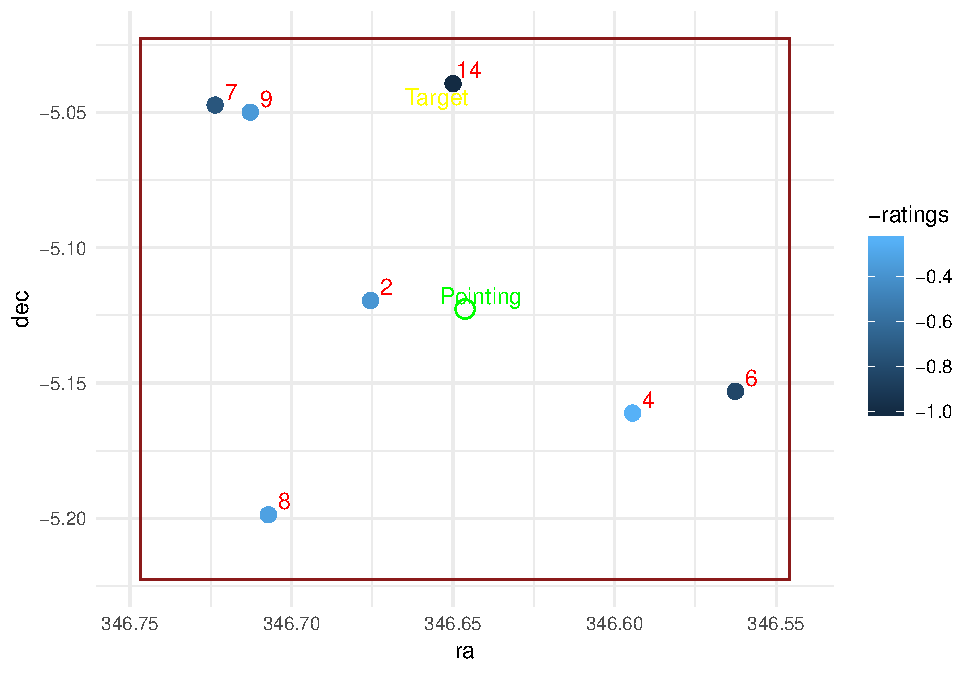
\includegraphics{Locus_example_files/figure-latex/locus_plot-1.pdf}

\newpage

\hypertarget{references}{%
\subsection*{References}\label{references}}
\addcontentsline{toc}{subsection}{References}

\hypertarget{refs}{}
\leavevmode\hypertarget{ref-Aguado2018}{}%
Aguado, D. S., Romina Ahumada, Andres Almeida, Scott F. Anderson, Brett
H. Andrews, Borja Anguiano, Erik Aquino Ortiz, et al. 2018. ``The
Fifteenth Data Release of the Sloan Digital Sky Surveys: First Release
of MaNGA Derived Quantities, Data Visualization Tools and Stellar
Library,'' December. \url{https://doi.org/10.3847/1538-4365/aaf651}.

\end{document}


